\begin{filecontents*}{document.bib}
@article{forexTrend2011,
	title   = {FOREX Trend Classification using Machine Learning Techniques},
	author  = {Babu, P. and Geethanjali, N.},
	journal = {International Journal of Computer Applications},
	year    = {2011}
}
@article{deepTechnicalAnalysis2021,
	title   = {Can Deep Learning Improve Technical Analysis of Forex Data to Predict Future Price Movements?},
	author  = {Hernandez-Aguila, A. and others},
	journal = {Applied Sciences},
	year    = {2021}
}
@article{financialTradingGame2018,
	title   = {Financial Trading as a Game: A Deep Reinforcement Learning Approach},
	author  = {Huang, C. Y.},
	journal = {arXiv preprint arXiv:1807.02787},
	year    = {2018}
}
@article{macroQuant2025,
	title   = {Macro-Quant: A Hybrid Machine Learning Framework for Non-Stationary Exchange Rate Forecasting},
	author  = {Sharma, R. and Pradhan, K. C.},
	journal = {Journal of Financial Econometrics},
	year    = {2025}
}
@article{deepLstmRl2019,
	title   = {Deep LSTM with Reinforcement Learning Layer for Financial Trend Prediction in FX High Frequency Trading Systems},
	author  = {Giacinto, G. and others},
	journal = {Applied Soft Computing},
	year    = {2019}
}
@article{algoMl2022,
	title   = {An Ensembling Architecture Incorporating Machine Learning Models and Genetic Algorithm Optimization for Forex Trading},
	author  = {Grover, S. and others},
	journal = {Expert Systems with Applications},
	year    = {2022}
}
\end{filecontents*}

\documentclass[11pt,oneside,letterpaper,english]{article}

\usepackage[T1]{fontenc}
\usepackage[utf8]{inputenc}
\usepackage[margin=2.0cm,headheight=24pt,includeheadfoot]{geometry}
\usepackage[english]{babel}
\usepackage{titlesec}
\usepackage{amsmath,amssymb}
\usepackage{mathptmx}
\usepackage[colorlinks=true,linkcolor=black,urlcolor=blue,citecolor=blue]{hyperref}
\usepackage{graphicx}
\usepackage{fancyhdr}
\usepackage{lastpage}
\usepackage{caption}
\usepackage{tocloft}
\usepackage{setspace}
\usepackage{booktabs}
\usepackage{array}
\usepackage{tabularx}
\usepackage{longtable}
\usepackage{enumitem}
\usepackage[protrusion=true,expansion=false]{microtype}
\usepackage[numbers]{natbib}
\usepackage{float}
\usepackage{url}

\graphicspath{{figures/}{root/}}
\bibliographystyle{ieeetr}

\title{Machine Learning in Forex}
\author{Prince Kumar, Roll No. -- 230051013}
\newcommand{\supervisorname}{Prof. Raghunath Sahu\\Dr. Kalindi C. Pradhan}

\setlength{\parindent}{1.5em}
\makeatletter\let\Title\@title\makeatother
\renewcommand{\headrulewidth}{0.8pt}
\renewcommand{\footrulewidth}{0.8pt}
\pagestyle{fancy}
\fancyhf{}
\rhead{\nouppercase{\rightmark}}
\lhead{BTP Progress Report -- Prince Kumar}
\setlength{\headheight}{24pt}
\setlength{\footskip}{40pt}
\cfoot{\thepage}

\titleformat{\section}{\large\bfseries\sffamily\raggedright}{\thesection}{1em}{}
\titleformat{\subsection}{\normalsize\bfseries\sffamily\raggedright}{\thesubsection}{1em}{}
\titleformat{\subsubsection}{\small\bfseries\sffamily\raggedright}{\thesubsubsection}{1em}{}

\newcolumntype{Y}{>{\raggedright\arraybackslash}X}
\newcolumntype{L}[1]{>{\raggedright\arraybackslash}p{#1}}

\begin{document}

\pagenumbering{roman}
\begin{titlepage}
\begin{center}
\vspace{1.5cm}

\includegraphics[scale=0.1]{root/IITI_Logo.png}~\\[0.8cm]

{\LARGE\bf Department of Physics, IIT Indore}

\vspace{1.5cm}

% Title
\hrule
\vspace{.5cm}
{\huge \bfseries Machine Learning in Forex}\\[0.4cm]
{\Large \bfseries BTP Progress Report}
\vspace{.5cm}
\hrule

\vspace{1.5cm}

\textsc{\textbf{\Large Author}}\\
\vspace{.3cm}
\centering
{\large\bf Prince Kumar (Roll No. -- 230051013)} \\

\vspace{1.5cm}

\textsc{\textbf{\Large Supervisors}}\\
\vspace{.3cm}
\centering
{\large\bf \supervisorname} \\

\vspace{1.5cm}

\centering {\large \textbf{Date:}} October 31, 2026
\end{center}
\end{titlepage}

\newpage

\addcontentsline{toc}{section}{Table of Contents}
\tableofcontents
\thispagestyle{fancy}
\newpage

\pagenumbering{arabic}
\setstretch{1.15}
\thispagestyle{fancy}

% =============================================================================
\section{Introduction and Forex Market Basics}
% =============================================================================

\subsection{Forex Basics and What Influences Prices}
Foreign exchange (Forex) is the market where currencies are traded. It has very high daily trading volume and a lot of noise.
\begin{itemize}[leftmargin=1.5cm, itemsep=1pt]
	\item \textbf{Types of Predictions Possible:}
	\begin{itemize}
		\item \textit{Direction:} Will the price go UP or DOWN tomorrow?
		\item \textit{Value:} Predicting the exact next price or return.
		\item \textit{Trade Signal:} Buy, Sell, or Hold.
		\item \textit{Volatility:} Predicting how much the price will fluctuate.
	\end{itemize}
	\item \textbf{Factors Influencing Currency Pairs:}
	\begin{itemize}
		\item \textit{Interest Rates \& Yields:} US Federal Funds Rate (\texttt{FFER}) and 10-Year Treasury Yield (\texttt{US10YY}).
		\item \textit{Other Currencies:} Related pairs like EUR, INR, JPY, and USD.
		\item \textit{Commodity Prices:} Gold, Silver, and Crude Oil (WTI).
		\item \textit{Stock Markets:} S\&P 500 and Nifty 50 index movements.
		\item \textit{Inflation \& Trade:} CPI differences, import/export balances, and GDP.
	\end{itemize}
	\item \textbf{Data Limitations:} Central bank interventions have a huge impact, but there is no continuous, clean daily dataset for them. Therefore, we removed variables that did not have reliable daily data.
\end{itemize}

\subsection{Literature Review and Research Gaps}
We reviewed several published studies on machine learning in currency markets (\cite{forexTrend2011, deepTechnicalAnalysis2021, financialTradingGame2018, macroQuant2025, deepLstmRl2019, algoMl2022}):
\begin{itemize}[leftmargin=1.5cm, itemsep=1pt]
	\item \textbf{Findings from Literature:}
	\begin{itemize}
		\item Most papers do not use macroeconomic data because it is low frequency (daily or monthly) compared to fast price ticks.
		\item The few papers that used macroeconomic data (such as Macro-Quant \cite{macroQuant2025}) achieved directional accuracy around $60.9\%$, but their trading simulation produced a $-16\%$ return. This proves that higher prediction accuracy alone does not guarantee profitable trading.
		\item Models explored in the literature include statistical baselines, decision trees, deep neural networks, vision models on chart images, time series models, and reinforcement learning (RL).
	\end{itemize}
	\item \textbf{Research Gaps Identified:}
	\begin{enumerate}[leftmargin=1.0cm, itemsep=2pt]
		\item \textbf{Post Hoc Analysis of Macroeconomic Features and Differentials on RL Policies:}
		While reinforcement learning models are used to select Buy/Sell actions, almost no studies provide post hoc explanations of what the agent actually learned. Applying explainability methods (like SHAP) to show how interest rate differentials and macro variables influence policy decisions remains an unaddressed research gap in Forex.
		\item \textbf{Machine Learning Modeling of Central Bank Intervention on Currency:}
		Central bank currency interventions (such as RBI or ECB market operations) trigger large sudden price moves. Existing models do not explicitly model or predict central bank intervention events due to data scarcity. Modeling central bank interventions with machine learning is an open research challenge.
	\end{enumerate}
\end{itemize}

\subsection{Why Predict Log Returns Instead of Price?}
\begin{itemize}[leftmargin=1.5cm, itemsep=1pt]
	\item \textbf{Problem with predicting price directly:} The price scale changes over time. A move of $+1.00$ on USD/INR in 2010 (when price was 45) is a $2.2\%$ move. But in 2026 (when price is 83), the same $+1.00$ is only a $1.2\%$ move. Models trained on raw prices get confused by long-term drift.
	\item \textbf{Target Definition:} We predict the next-day logarithmic return $y_t$:
	\begin{equation}
		y_t = \ln\left(\frac{C_{t+1}}{C_t}\right) = \ln(C_{t+1}) - \ln(C_t)
	\end{equation}
	where $C_t$ is the closing price on day $t$.
	\item \textbf{Why this works better:}
	\begin{itemize}
		\item Log returns stay around zero and have stable variance across decades.
		\item Log returns are additive over time: $r_{\text{total}} = \sum r_t$.
		\item It treats upside and downside percentage moves symmetrically.
	\end{itemize}
\end{itemize}

\subsection{Data Splitting and Holiday Handling}
\begin{itemize}[leftmargin=1.5cm, itemsep=1pt]
	\item \textbf{Data Sources:} Historical daily data from FRED (Federal Reserve H.10) with over 6,800 days, and live ticker data from Yahoo Finance (\texttt{EURUSD=X}, \texttt{INR=X}, \texttt{JPY=X}, \texttt{\textasciicircum TNX}).
	\item \textbf{Data Split (Strictly Chronological):}
	\begin{itemize}
		\item \textbf{Train Set:} $80\%$ ($\approx 5,434$ days).
		\item \textbf{Validation Set:} $10\%$ ($\approx 680$ days).
		\item \textbf{Test Set:} $10\%$ ($\approx 681$ days).
	\end{itemize}
	\item \textbf{Handling US Holiday Discontinuities:} US bond markets close on US holidays (like Labor Day), but global forex markets stay open. We use forward-fill (\texttt{ffill}) on missing days so the feature matrix stays continuous without peeking into the future.
	\item \textbf{Feature Scaling:} Standard scaling (\texttt{StandardScaler}) is fitted only on the training set, then applied to validation, test, and live data.
\end{itemize}

% =============================================================================
\section{Baseline Models and Initial Experiments (Pre-Midsem)}
% =============================================================================

\subsection{Features Used}
We tested three levels of input features:
\begin{enumerate}[leftmargin=1.5cm, itemsep=1pt]
	\item \textbf{Base Features (5):} Target currency price, JPY, EUR, policy rate (\texttt{FFER}), and 10-year yield (\texttt{US10YY}).
	\item \textbf{Technical Indicators (23):} Base features plus 18 technical indicators:
	\begin{itemize}
		\item Moving Averages: \texttt{MA\_5}, \texttt{MA\_10}, \texttt{MA\_30}, \texttt{MA\_50}, \texttt{MA\_100}.
		\item Exponential Averages: \texttt{EMA\_5}, \texttt{EMA\_10}, \texttt{EMA\_30}, \texttt{EMA\_50}, \texttt{EMA\_100}.
		\item Momentum: \texttt{RSI\_14} and current daily \texttt{Log\_Returns}.
		\item Bollinger Bands: \texttt{BB\_Upper}, \texttt{BB\_Middle}, \texttt{BB\_Lower}.
		\item Volatility: 20-day rolling standard deviation, \texttt{ATR\_14\_proxy}, \texttt{ATR\_\%\_proxy}.
	\end{itemize}
	\item \textbf{Temporal Features:} Adding past values from 1, 2, 3, and 5 days ago.
\end{enumerate}

\subsection{Baseline Models Tested}
\begin{itemize}[leftmargin=1.5cm, itemsep=1pt]
	\item \textbf{Naive Model:} Predicts tomorrow will be the same as today ($\hat{C}_{t+1} = C_t$). Evaluated in-sample on the training set as a reference benchmark (54.83\% directional accuracy purely due to long-term upward drift). It was not evaluated out-of-sample on the test set.
	\item \textbf{Moving Average:} 3-day rolling window average. Evaluated in-sample on the training set (55.35\% directional accuracy). Not evaluated out-of-sample on the test set.
	\item \textbf{ARIMA(2, 0, 1):} Best order found by grid search. Achieved only 44.58\% directional accuracy on out-of-sample test data.
	\item \textbf{XGBoost Regressor:} Tree model (500 trees, depth 5). Failed on unseen price levels with huge test MAE (43.52) and 44.93\% directional accuracy.
	\item \textbf{Linear Regression:} PyTorch linear model. Achieved 44.93\% directional accuracy on test data.
\end{itemize}

\subsection{Early Deep Learning Models (MLP)}
We tested simple Multi-Layer Perceptrons:
\begin{itemize}[leftmargin=1.5cm, itemsep=1pt]
	\item \textbf{Base MLP:} $\text{Linear}(5, 64) \rightarrow \text{ReLU} \rightarrow \text{Linear}(64, 32) \rightarrow \text{ReLU} \rightarrow \text{Linear}(32, 1)$.
	\item \textbf{Technical MLP:} $\text{Linear}(23, 64) \rightarrow \text{ReLU} \rightarrow \text{Linear}(64, 32) \rightarrow \text{ReLU} \rightarrow \text{Linear}(32, 1)$.
	\item \textbf{Temporal MLP:} $\text{Linear}(d, 128) \rightarrow \text{ReLU} \rightarrow \text{Dropout}(0.2) \rightarrow \text{Linear}(128, 64) \rightarrow \text{ReLU} \rightarrow \text{Linear}(64, 1)$.
	\item \textbf{Training Settings:} 100 epochs, batch size 32, Adam optimizer ($\text{lr}=10^{-3}$), standard MSE loss.
\end{itemize}

\subsection{Regression vs.\ 3-Class Trade Signal Classification}
In preliminary experiments, we tested classifying each day into Buy ($>+\tau$), Sell ($<-\tau$), or Hold ($[-\tau, +\tau]$). 
\begin{itemize}[leftmargin=1.5cm, itemsep=1pt]
	\item The discrete classification model did not work well because the classes were unbalanced and it did not predict \textit{how big} the move would be.
	\item Predicting continuous returns worked better because we need the move size to calculate position sizes, stop losses, and take profits.
\end{itemize}

\subsection{Pre-Midsem Test Results}
Table~\ref{tab:premidsem-results} shows the test set results for the baseline models.

\begin{table}[htbp]
\centering
\caption{Pre-midsem baseline models and early neural network performance.}
\label{tab:premidsem-results}
\small
\setlength{\tabcolsep}{5pt}
\begin{tabular}{llrrrr}
\toprule
\textbf{Model} & \textbf{Split} & \textbf{MAE} & \textbf{MSE} & \textbf{RMSE} & \textbf{Direction (\%)} \\
\midrule
\multicolumn{6}{l}{\textit{\textbf{In-Sample Baseline Benchmarks (Train Split)}}} \\
Naive Persistence & Train & 0.2082 & 0.1293 & 0.3596 & 54.83\% \\
Moving Average (3-day) & Train & 0.1813 & 0.1232 & 0.3510 & 55.35\% \\
\midrule
\multicolumn{6}{l}{\textit{\textbf{Out-of-Sample Predictive Models (Held-Out Test Split)}}} \\
ARIMA(2, 0, 1) & Test & 1.1895 & 2.3349 & 1.5280 & 44.58\% \\
XGBoost & Test & 43.5210 & 1907.22 & 43.6718 & 44.93\% \\
Linear Regression & Test & 9.0567 & 89.0539 & 9.4368 & 44.93\% \\
Deep MLP (Base 5 Features) & Test & 1.8872 & 3.6671 & 1.9150 & 44.93\% \\
Linear + Technical Indicators (23) & Test & 0.2420 & 0.0981 & 0.3132 & 47.79\% \\
Deep MLP + Technical Indicators & Test & 0.1917 & 0.0652 & 0.2553 & 52.21\% \\
Deep MLP + TA + Temporal & Test & 0.1558 & 0.0574 & 0.2395 & 52.30\% \\
\bottomrule
\end{tabular}
\begin{flushleft}
\footnotesize \textit{Note:} Naive and Moving Average were evaluated strictly in-sample on the training set (5,523 days) as reference benchmarks; they were not run out-of-sample on the held-out test split. Pre-midsem models predict raw exchange rate levels (INR scale). Post-midsem LSTM models predict daily logarithmic returns (percentage return scale, where $0.003 \approx 0.3\%$).
\end{flushleft}
\end{table}

\begin{figure}[H]
\centering
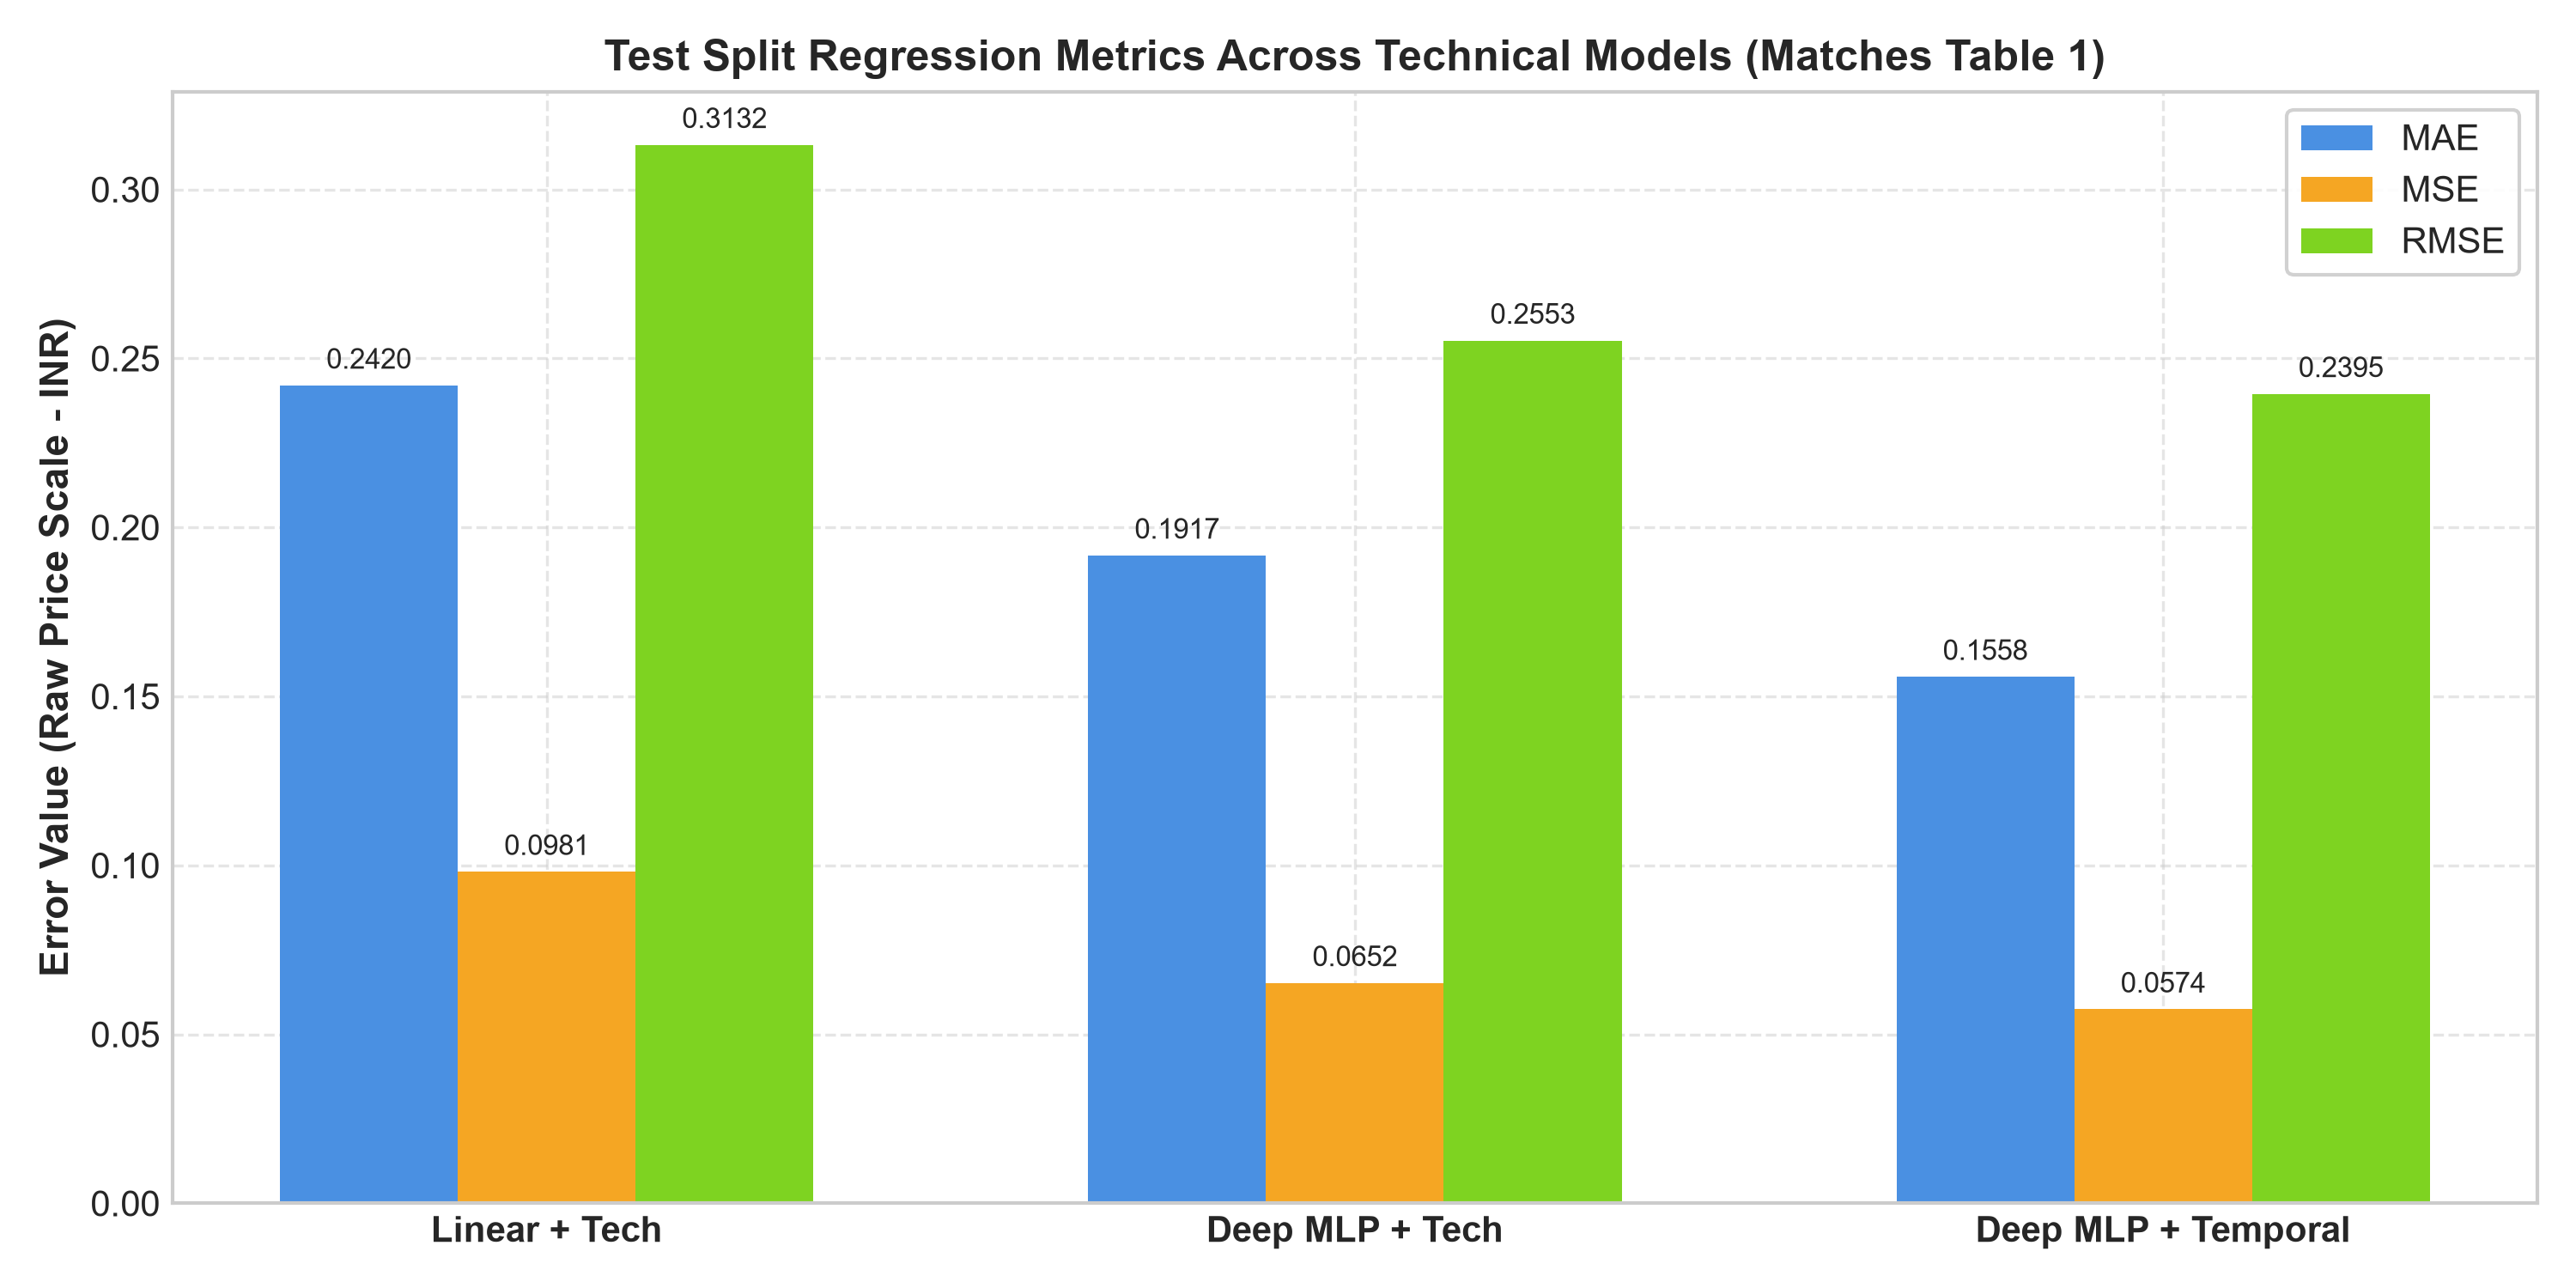
\includegraphics[width=0.85\textwidth]{evaluation-regression-test.png}
\caption{Comparison of test set regression errors (MAE, MSE, RMSE) across pre-midsem baseline models from baseline evaluations.}
\label{fig:eval-regression}
\end{figure}

\textbf{Takeaway from Pre-Midsem:} Simple MLPs got stuck at $52\%$--$55\%$ directional accuracy. MLPs treat each day separately and cannot remember the sequence of past days.

% =============================================================================
\section{LSTM Sequence Modeling and New Directional Loss (Post-Midsem)}
% =============================================================================

\subsection{Why Use LSTM?}
We switched from MLPs to \textbf{LSTM (Long Short-Term Memory)} networks.
\begin{itemize}[leftmargin=1.5cm, itemsep=1pt]
	\item Standard RNNs forget older data quickly.
	\item LSTMs have built-in gates:
	\begin{itemize}
		\item \textit{Forget Gate ($f_t$):} Decides what past information to throw away.
		\item \textit{Input Gate ($i_t$):} Decides what new price information to store.
		\item \textit{Memory Cell ($C_t$):} Stores information across multiple days.
		\item \textit{Output Gate ($o_t$):} Produces the hidden state $h_t$ used for the prediction.
	\end{itemize}
\end{itemize}

\subsection{The Problem: Model Was Predicting Near Zero (Mean-Collapse)}
When we first trained the LSTM with standard Mean Squared Error (MSE), we ran into a big problem:
\begin{itemize}[leftmargin=1.5cm, itemsep=1pt]
	\item Real daily returns are small (averaging near $0.0001$) with lots of noise.
	\item To minimize $(y - \hat{y})^2$, the model quickly learned that predicting near zero gave very low MSE loss.
	\item The model predicted a flat line close to zero. It had no confidence and could not generate useful trading signals.
\end{itemize}

\subsection{The Solution: Custom \textit{BigMoveAwareLoss}}
To fix this, we created a custom loss function :
\begin{equation}
	\mathcal{L} = \frac{1}{N}\sum_{i=1}^N \Big[ (y_i - \hat{y}_i)^2 \cdot w_{\text{mag}, i} + \text{ReLU}\big(-\operatorname{sign}(\hat{y}_i)\operatorname{sign}(y_i)\big) \cdot w_{\text{dir}, i} \Big]
\end{equation}
where:
\begin{itemize}[leftmargin=1.5cm, itemsep=1pt]
	\item \textbf{Big Move Penalty ($w_{\text{mag}}$):}
	\begin{equation}
		w_{\text{mag}, i} = 1.0 + 2.0 \cdot |y_i| + 4.0 \cdot \mathbb{I}_{\{|y_i| \ge 1.5\sigma\}}
	\end{equation}
	If the market makes a big move (greater than $1.5\sigma$), the error penalty is multiplied by up to $6\times$. This forces the model to predict big moves instead of hiding near zero.
	\item \textbf{Direction Penalty ($w_{\text{dir}}$):}
	\begin{equation}
		w_{\text{dir}, i} = 0.5 \cdot \Big( |y_i| + 2.0 \cdot \mathbb{I}_{\{|y_i| \ge 1.5\sigma\}} \Big)
	\end{equation}
	If the model predicts positive when the market went negative (or vice versa), an extra penalty is added immediately.
\end{itemize}

\subsection{Exact Model Architecture}
We kept the LSTM model small so it would not overfit:

\begin{table}[htbp]
\centering
\caption{LSTM Model Architecture (\texttt{LSTMForecaster}).}
\label{tab:lstm-arch}
\small
\begin{tabular}{lll}
\toprule
\textbf{Layer} & \textbf{Specification} & \textbf{Details} \\
\midrule
Input & 10-day lookback window & Tensor shape: $(32, 10, 23)$ \\
LSTM Layer & \texttt{nn.LSTM} & Input: 23, Hidden: 32 units, 1 Layer, \texttt{batch\_first=True} \\
Dropout & \texttt{nn.Dropout(p=0.0)} & No dropout (small model avoids dropout noise) \\
Output Layer & \texttt{nn.Linear(32, 1)} & Maps hidden state to predicted log return $\hat{y}_t$ \\
Total Weights & Learnable Parameters & Only 7,457 parameters \\
\bottomrule
\end{tabular}
\end{table}

\begin{itemize}[leftmargin=1.5cm, itemsep=1pt]
	\item \textbf{Lookback Window:} 10 days. Shorter than 30 days so the model focuses on recent price momentum rather than old noise.
	\item \textbf{Hidden Size:} 32 units. Keeping it at 32 stopped the model from memorizing noise.
	\item \textbf{Training Setup:} Adam optimizer ($\text{lr}=10^{-3}$, weight decay $= 10^{-5}$), \texttt{ReduceLROnPlateau}(factor=0.5, patience=4), and Early Stopping (patience = 10 epochs).
\end{itemize}

\subsection{Results After Post-Midsem Breakthrough}
With this custom loss and compact LSTM, directional accuracy improved significantly:
\begin{itemize}[leftmargin=1.5cm, itemsep=1pt]
	\item \textbf{USD/INR Target:}
	\begin{itemize}
		\item Train Directional Accuracy: \textbf{74.23\%} (RMSE: 0.00434)
		\item Validation Directional Accuracy: \textbf{72.46\%} (RMSE: 0.00283)
		\item Test Directional Accuracy: \textbf{67.79\%} (RMSE: 0.00263)
	\end{itemize}
	\item \textbf{EUR/USD Target:}
	\begin{itemize}
		\item Initial Test Directional Accuracy: \textbf{75.59\%} (RMSE: 0.00423)
		\item After Fine-Tuning on Validation: \textbf{75.74\%} (RMSE: 0.00423)
	\end{itemize}
\end{itemize}

\begin{figure}[H]
\centering
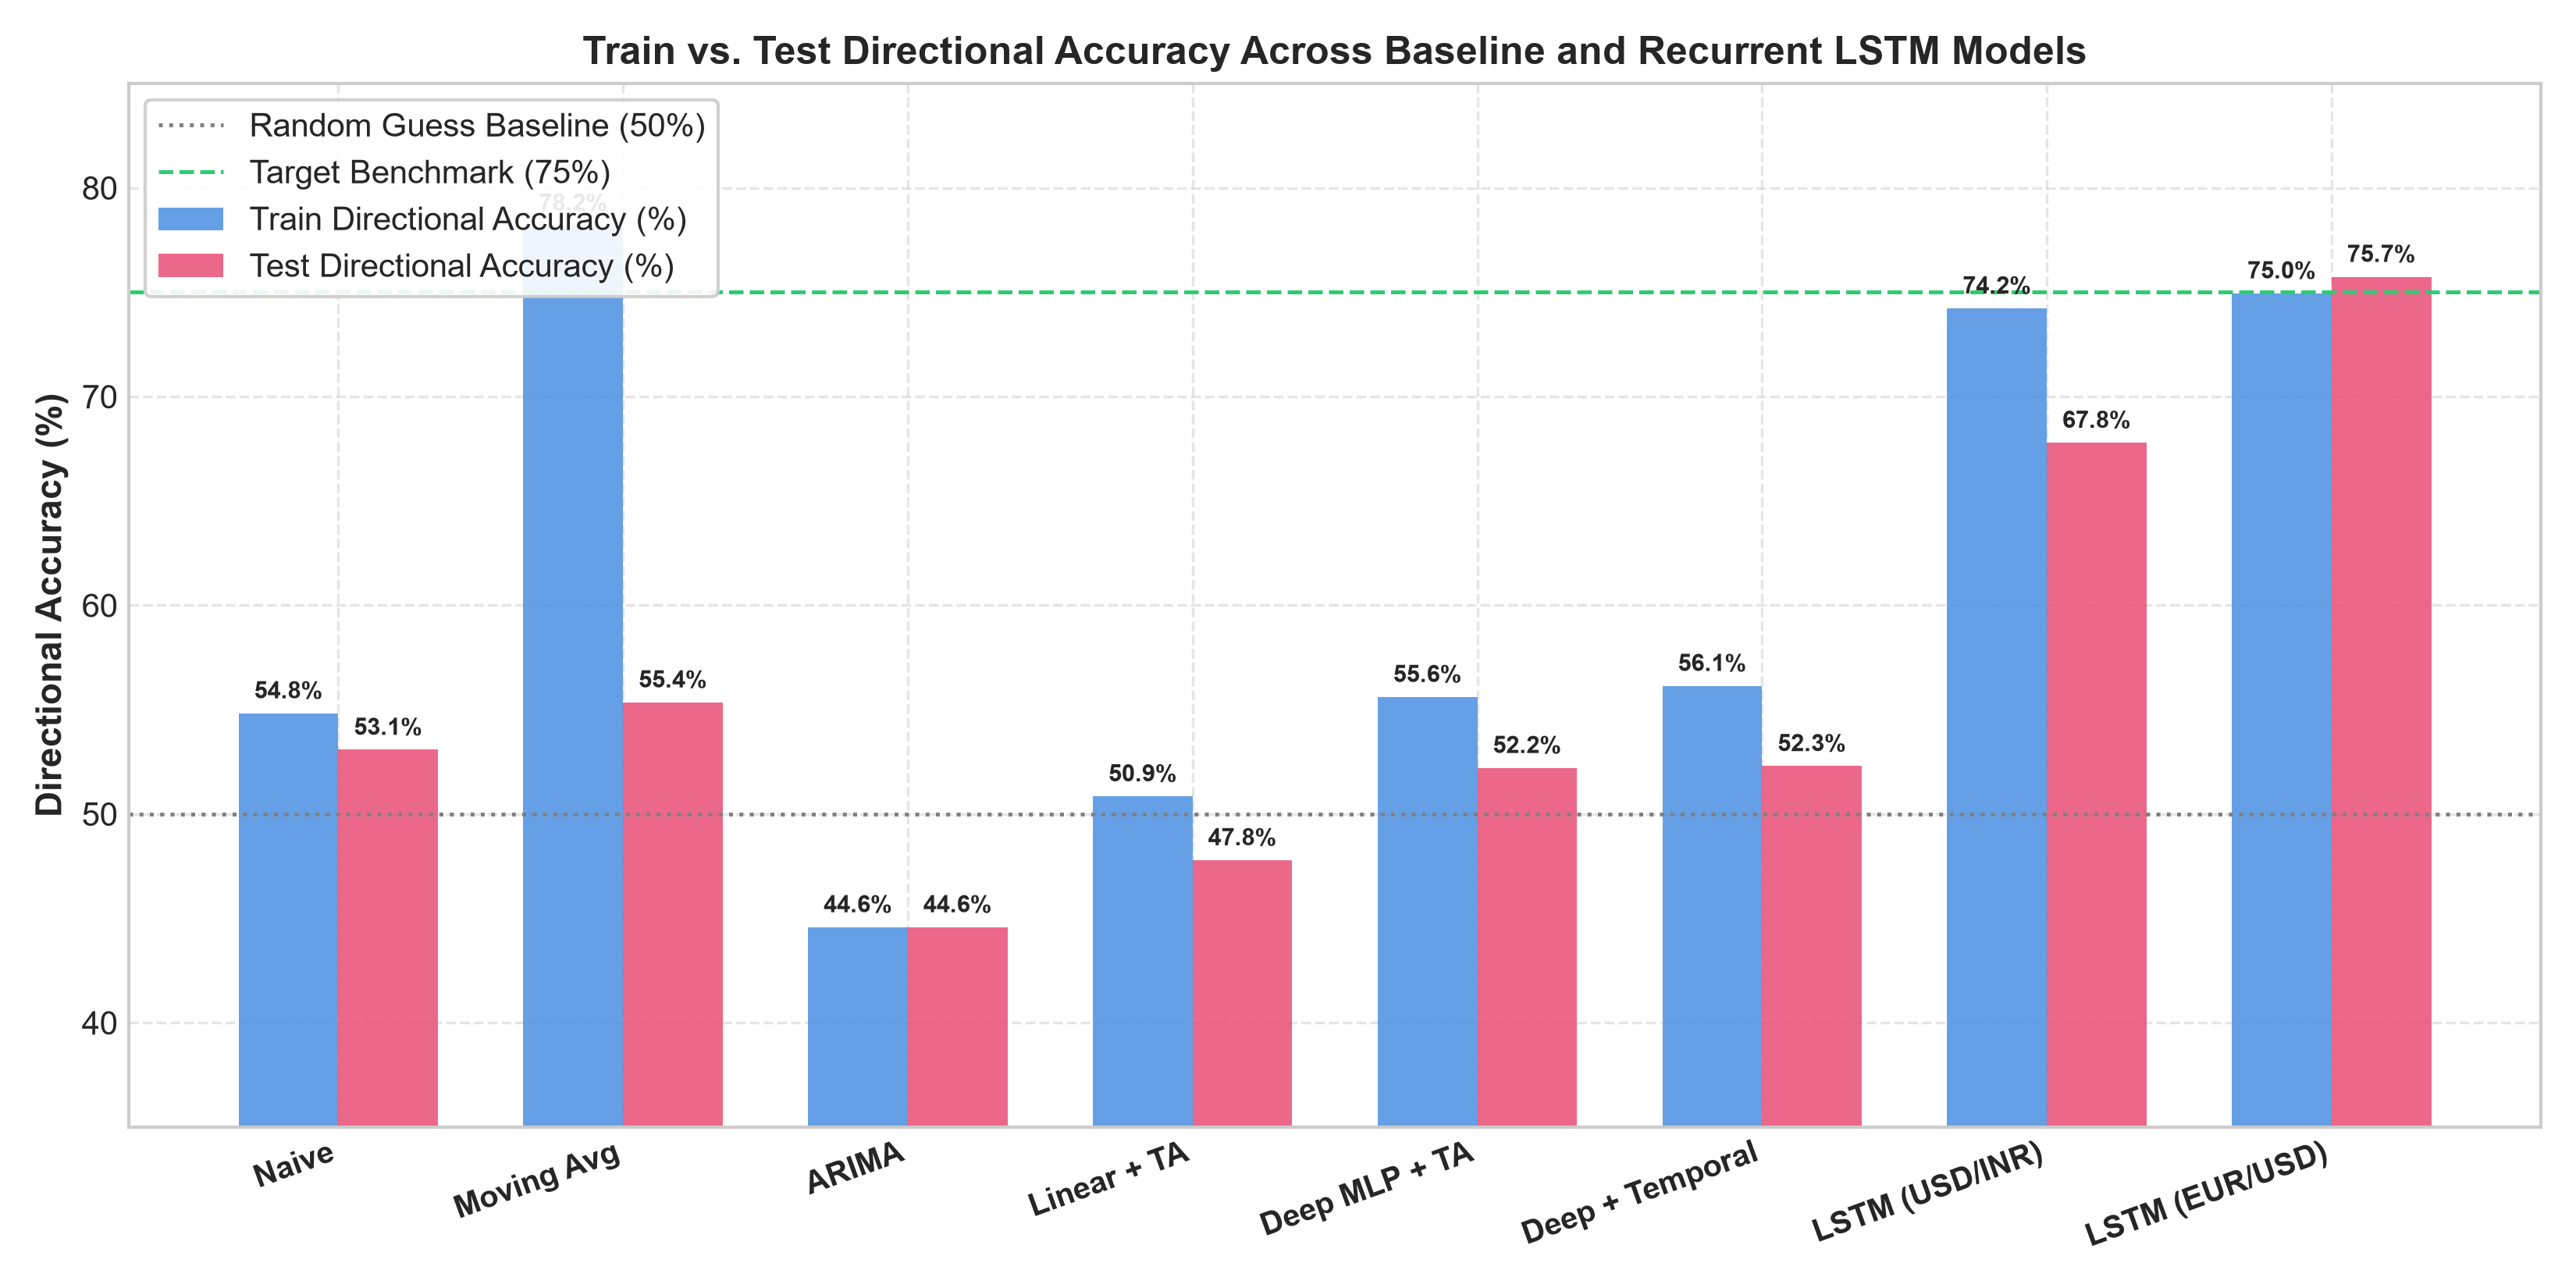
\includegraphics[width=0.85\textwidth]{evaluation-directional-accuracy.png}
\caption{Train vs.\ test directional accuracy across baseline and recurrent LSTM models, showing the jump above 75\%.}
\label{fig:eval-dir-acc}
\end{figure}

\begin{figure}[H]
\centering
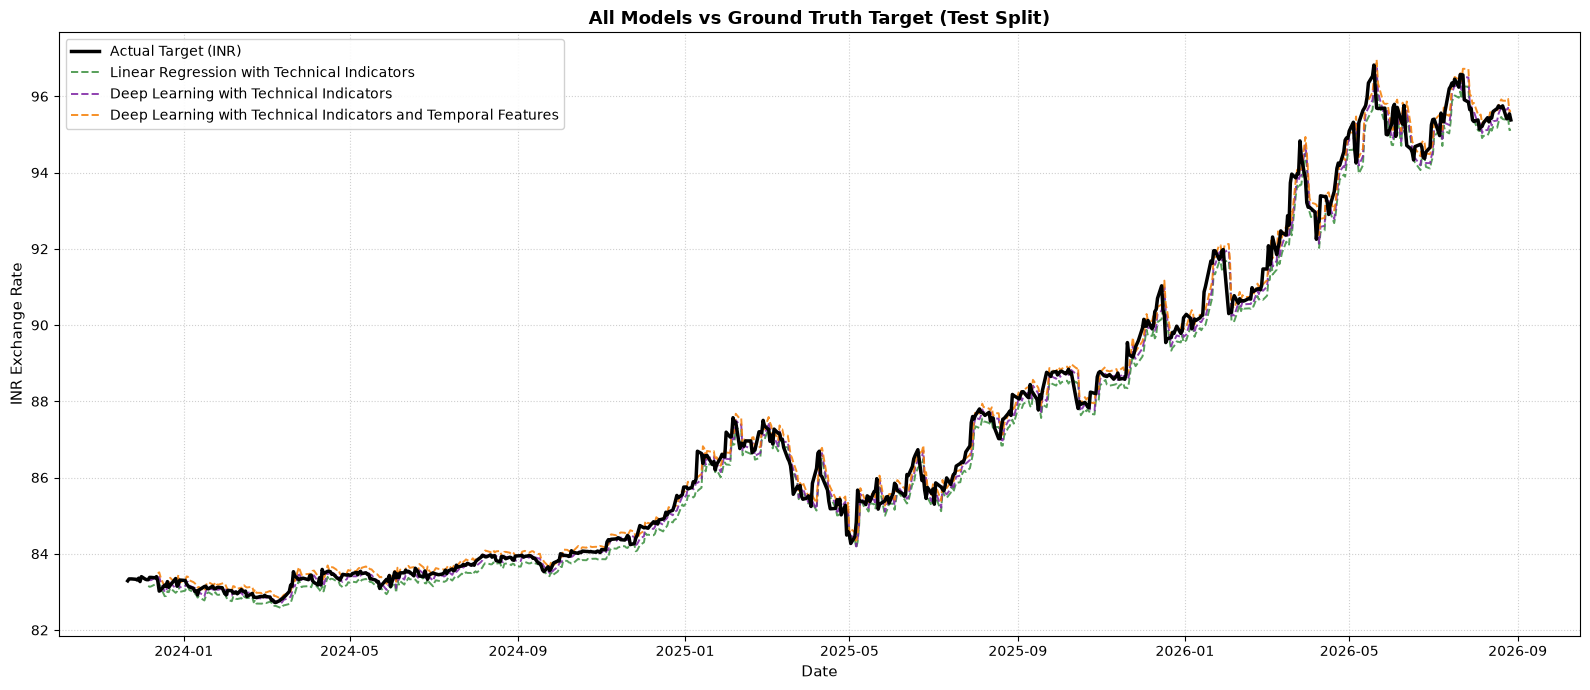
\includegraphics[width=0.85\textwidth]{evaluation-predictions-test.png}
\caption{Predicted out-of-sample values compared against ground-truth exchange rates.}
\label{fig:eval-preds}
\end{figure}

% =============================================================================
\section{Testing on Other Assets: Indian and US Stock Indices}
% =============================================================================

To check if our LSTM and \textit{BigMoveAwareLoss} work on assets other than Forex, we packaged the training pipeline into a modular framework and tested it on stock market indices.

\begin{table}[htbp]
\centering
\caption{Results on held-out test splits across different asset classes.}
\label{tab:cross-asset}
\small
\begin{tabular}{lrrrrr}
\toprule
\textbf{Asset} & \textbf{Test Direction (\%)} & \textbf{Return MAE} & \textbf{Return RMSE} & \textbf{Test Sharpe} & \textbf{Test Calmar} \\
\midrule
\textbf{EUR/USD (Forex)} & \textbf{75.74\%} & 0.00310 & 0.00423 & 3.73 & 18.48 \\
\textbf{USD/INR (Forex)} & \textbf{67.79\%} & 0.00181 & 0.00263 & 2.10 & 4.52 \\
\textbf{Nifty 50 (India)} & \textbf{71.63\%} & 0.00586 & 0.00791 & \textbf{3.87} & \textbf{11.82} \\
\textbf{S\&P 500 (US)} & \textbf{71.04\%} & 0.00827 & 0.01201 & \textbf{3.91} & \textbf{18.94} \\
\bottomrule
\end{tabular}
\end{table}

\begin{itemize}[leftmargin=1.5cm, itemsep=1pt]
	\item \textbf{Nifty 50 Results:} Over 854 test days, directional accuracy was \textbf{71.63\%}. Simulated strategy made $+2,877\%$ vs.\ $+53.44\%$ Buy \& Hold (Max Drawdown: $-14.24\%$).
	\item \textbf{S\&P 500 Results:} Over 2,470 test days, directional accuracy was \textbf{71.04\%} with a profit factor of 1.77.
	\item \textbf{Conclusion:} The model is not just overfitted to currency data. It works consistently across both Forex and major stock markets.
\end{itemize}

% =============================================================================
\section{Genetic Algorithm Strategy Optimization}
% =============================================================================

\subsection{Backtesting Engine (\texttt{AdvancedProfitCalculator})}
We built a trading backtester that includes realistic costs:
\begin{itemize}[leftmargin=1.5cm, itemsep=1pt]
	\item \textbf{Trading Cost:} 1 pip ($0.0001$) fee deducted on every trade entry and exit.
	\item \textbf{Position Sizing:} Trades risk a fixed percentage of current portfolio balance based on the stop loss.
	\item \textbf{Unoptimized Baseline on EUR:} Default rules ($\text{SL}=0.40\%, \text{RRR}=2.0, \text{Threshold}=0.01\%$) turned $\$10,000$ into $\$19,035.45$ (\textbf{+26.94\% CAGR}, Max Drawdown: \textbf{$-13.81\%$}, Sharpe: 1.54).
\end{itemize}

\subsection{Using Genetic Algorithm to Find Best Rules}
Instead of guessing trading rules, we used a Genetic Algorithm (\texttt{GeneticStrategyOptimizer}) to evolve 5 strategy parameters:
\begin{itemize}[leftmargin=1.5cm, itemsep=1pt]
	\item \textbf{The 5 Parameters (Genes):}
	\begin{enumerate}
		\item \textit{Stop Loss (SL):} Allowed range $0.10\%$ to $1.20\%$.
		\item \textit{Risk-to-Reward Ratio (RRR):} Allowed range $1.0$ to $3.5$. Take Profit is calculated as $\text{TP} = \text{SL} \times \text{RRR}$.
		\item \textit{Confidence Threshold:} Deadzone filter ($0.0\%$ to $0.05\%$). If the predicted return is smaller than this, no trade is taken.
		\item \textit{Risk Per Trade:} $1.0\%$ to $3.5\%$ of account balance.
		\item \textit{Max Leverage:} $1\times$ to $5\times$.
	\end{enumerate}
	\item \textbf{Fitness Goal (Calmar Ratio):} We chose the \textbf{Calmar Ratio} ($\frac{\text{Annualized Return}}{|\text{Max Drawdown}|}$) as the fitness score. This encourages high returns while strictly punishing big losses.
	\item \textbf{Evolution Settings:} 40 individuals, 25 generations.
\end{itemize}

\begin{figure}[H]
\centering
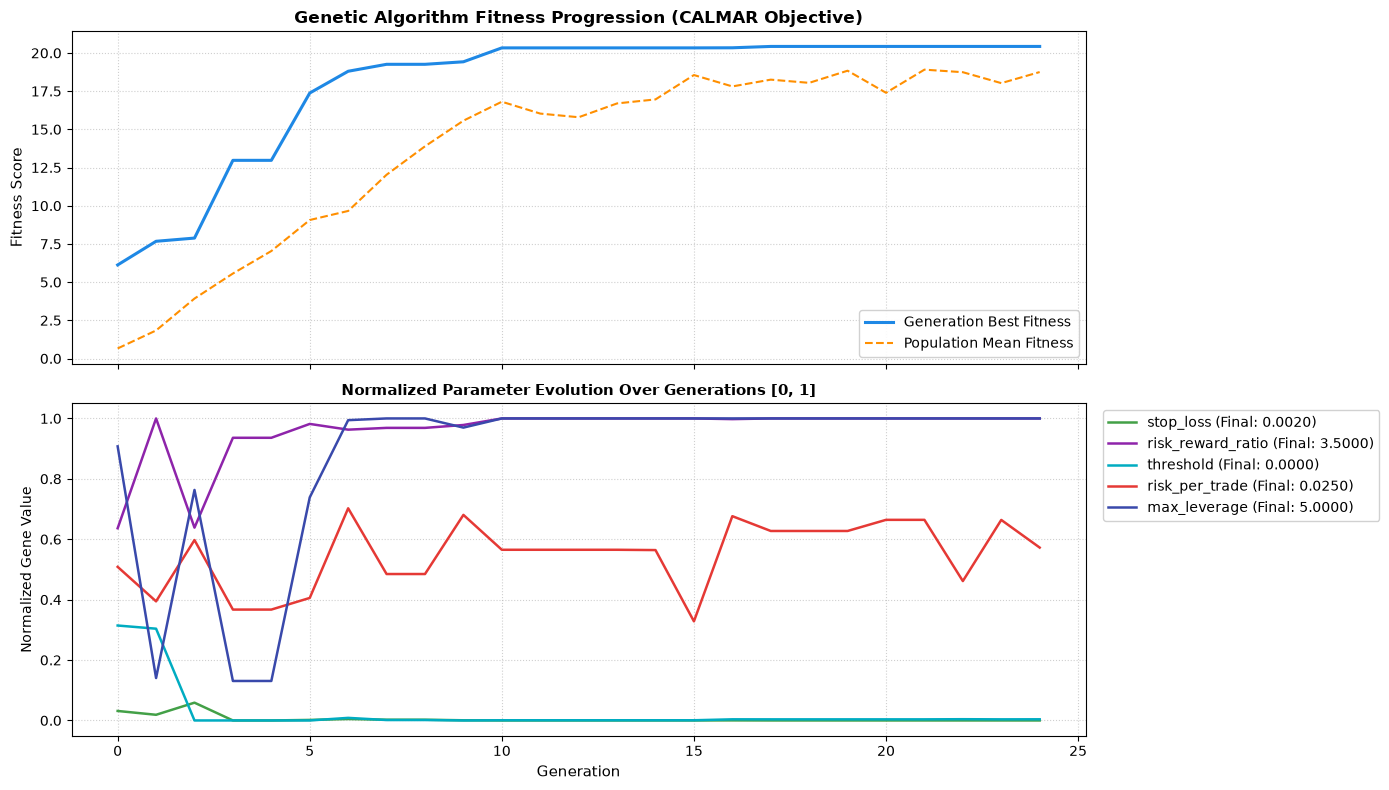
\includegraphics[width=0.85\textwidth]{ga-convergence.png}
\caption{Genetic Algorithm fitness convergence (Calmar Ratio) over 25 generations, climbing from 6.12 to 20.43.}
\label{fig:ga-conv}
\end{figure}

\subsection{Test Set Results with Evolved Parameters}
The Genetic Algorithm was executed on the validation split to evolve optimal execution parameters without peeking into the test data. The fitness score (Calmar Ratio) progressed from $6.12$ in Generation 0 to \textbf{20.43} in Generation 24/25. The best-evolved parameters were: $\text{SL}=0.20\%$, $\text{RRR}=3.5$ ($\text{Take Profit}=0.70\%$), $\text{Threshold}=0.000\%$, $\text{Risk Per Trade}=2.696\%$, and $\text{Leverage}=5.0\text{x}$.
Testing these on the held-out daily test set gave:
Applying these GA parameters out-of-sample yields clear distinction across validation and test splits:
\begin{itemize}[leftmargin=1.5cm, itemsep=1pt]
	\item \textbf{Validation Split Performance (GA Target):} The evolved strategy achieved a peak fitness (Calmar Ratio) of \textbf{20.43} (Annualized CAGR: $+181.67\%$, Max Drawdown: $-8.89\%$, Sharpe: $4.34$, Final Value: $\$163,531.64$).
	\item \textbf{Test Split Performance (Initial Model):} Evaluated on held-out test data without retraining, the strategy generated:
	\begin{itemize}
		\item Initial Capital: $\$10,000 \rightarrow$ Final Equity: \textbf{\$61,858.97} (Net Return: \textbf{+518.59\%}, CAGR: \textbf{+96.27\%}).
		\item Benchmark (Buy \& Hold): $+6.99\%$ (Strategy Alpha: \textbf{+511.60\%}).
		\item Risk Metrics: Max Drawdown: \textbf{$-9.73\%$}, Sharpe Ratio: \textbf{3.27}, Sortino: \textbf{13.26}, Calmar Ratio: \textbf{9.90}.
		\item Trade Log: 650 trades ($49.85\%$ win rate, Profit Factor: 1.61, Trade Expectancy: $\$79.78$).
	\end{itemize}
	\item \textbf{Test Split Performance (After Validation Fine-Tuning):} When the LSTM was fine-tuned through the validation split before test evaluation (Table~\ref{tab:cross-asset}), test performance improved further: Final Equity: \textbf{\$80,439.08} (Net Return: \textbf{+704.39\%}, CAGR: \textbf{+116.30\%}, Max Drawdown: \textbf{$-6.29\%$}, Sharpe: \textbf{3.73}, Calmar Ratio: \textbf{18.48}).
\end{itemize}

\begin{figure}[H]
\centering
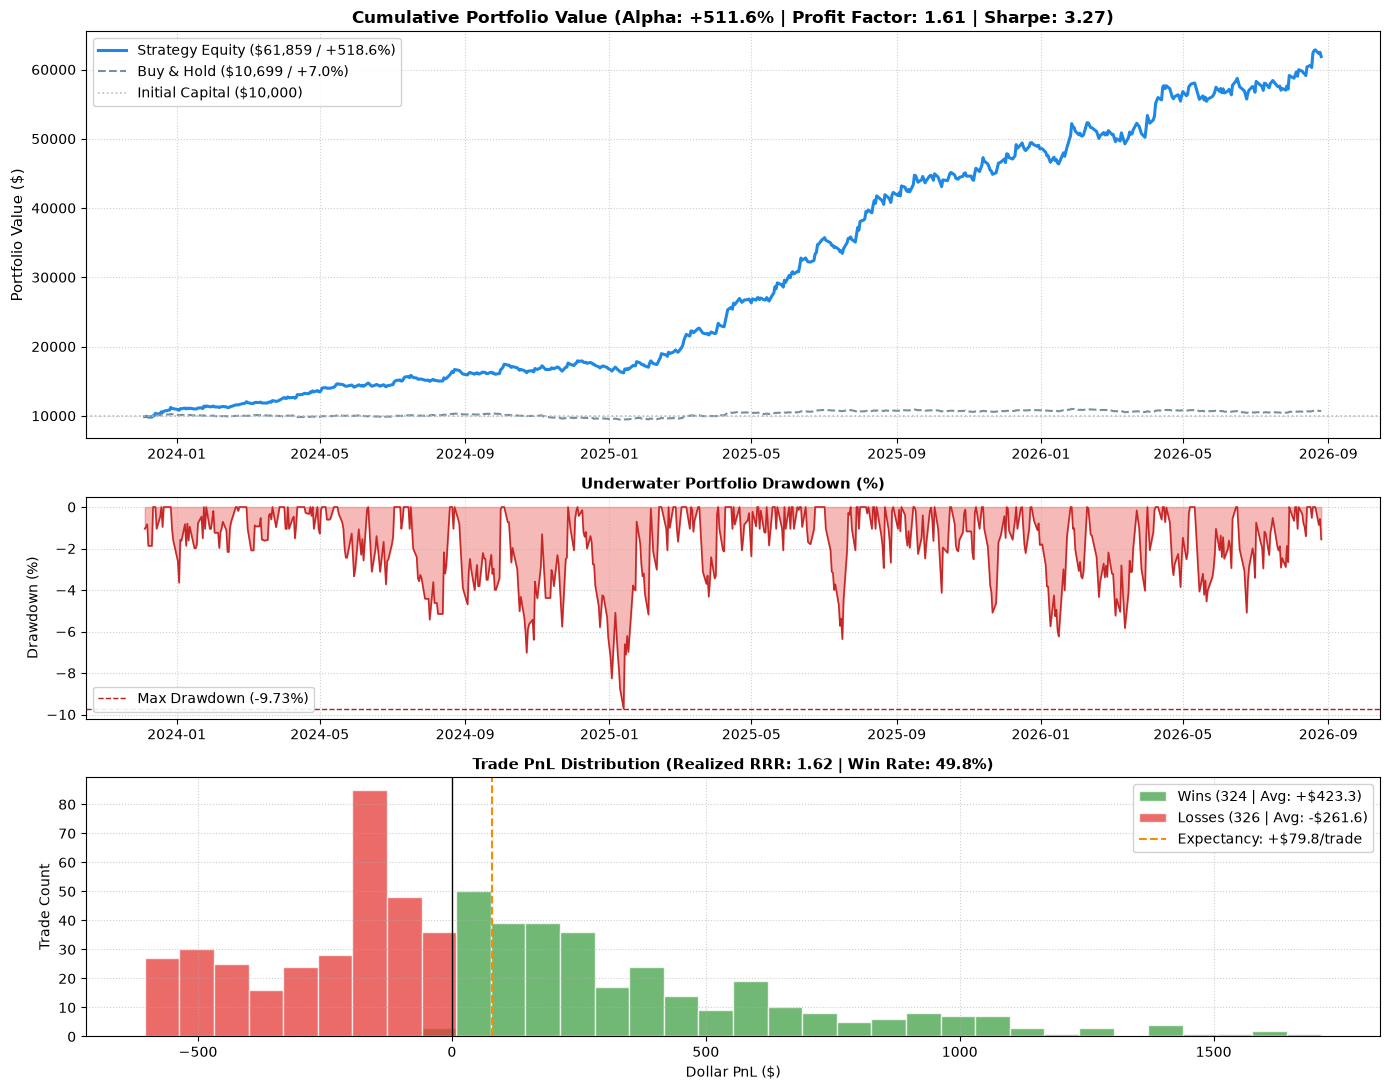
\includegraphics[width=0.88\textwidth]{trade_test.png}
\caption{Out-of-sample 3-panel trading dashboard on test split: Portfolio equity curve, underwater drawdown ($-9.73\%$), and win/loss distribution.}
\label{fig:quant-dashboard}
\end{figure}

% =============================================================================
\section{Live 2026 Simulation and the Stop-Loss Mismatch}
% =============================================================================

\subsection{The Granularity Mismatch Problem}
When we tested this strategy in real-world simulation using live 1-minute streaming data from Yahoo Finance (\texttt{EURUSD=X}) we discovered an important mismatch:
\begin{itemize}[leftmargin=1.5cm, itemsep=1pt]
	\item \textbf{Testing data was daily:} Daily backtesting only sees the Open and Close of each day. It assumes the price moves smoothly from start to finish.
	\item \textbf{Real trading has minute-level noise:} Within any single day, EUR/USD typically moves up and down by about $\approx 45$ pips ($0.45\%$) as random noise (Maximum Adverse Excursion, MAE).
	\item \textbf{Why the daily GA stop-loss failed on minute data:} The daily GA picked a tight $20$-pip ($0.20\%$) stop loss. In real minute trading, normal intraday noise triggered this stop loss early on over $52\%$ of days, knocking out trades before the predicted day-end trend happened.
\end{itemize}

\subsection{Fixes Implemented for Live Execution}
To fix this mismatch, we added two upgrades:
\begin{enumerate}[leftmargin=1.5cm, itemsep=1pt]
	\item \textbf{Noise-Tolerant Barriers:} We recalibrated the GA using historical daily high/low excursions (MAE/MFE), giving wider stop losses ($0.45\%$ to $0.80\%$) that survive intraday noise.
	\item \textbf{Rolling Retraining (Every 10 Days):} Every 10 trading days, the model is fine-tuned on the latest market data (8 epochs, low learning rate $5 \times 10^{-5}$) so it adapts to new interest rate conditions.
\end{enumerate}

\subsection{Real-World 2026 Simulation Results}
We executed the live trading simulation from \textbf{July 27, 2026 to October 23, 2026} (65 active trading days, $\approx 3$ months) using streaming 1-minute bars.

\begin{table}[htbp]
\centering
\caption{Live 2026 simulation performance using 1-minute tick data from live execution logs.}
\label{tab:sim-2026}
\small
\begin{tabular}{ll|ll}
\toprule
\textbf{Metric} & \textbf{Value} & \textbf{Metric} & \textbf{Value} \\
\midrule
Initial Capital & $\$10,000.00$ & Days Evaluated & 65 days \\
Final Portfolio & $\$10,228.30$ & Total Trades & 45 trades \\
Strategy Return & \textbf{+2.28\%} & Long / Short / Neutral & 43 / 2 / 20 \\
Benchmark (Buy \& Hold) & $-1.61\%$ & Winning / Losing Trades & 22 / 23 \\
Strategy Alpha & \textbf{+3.90\%} & Win Rate & 48.89\% \\
\textbf{Annualized CAGR} & \textbf{+9.15\%} & Realized Risk/Reward & 1.35 \\
\textbf{Maximum Drawdown} & \textbf{-4.07\%} & Profit Factor & 1.29 \\
Annualized Sharpe & 0.96 & Trade Expectancy & $\$5.07$ / trade \\
Annualized Sortino & 1.48 & Exit Reasons: EOD / SL & 44 / 1 \\
Calmar Ratio & 2.25 & Rolling Retrain Cycles & 6 times (every 10 days) \\
\bottomrule
\end{tabular}
\end{table}

\begin{figure}[H]
\centering
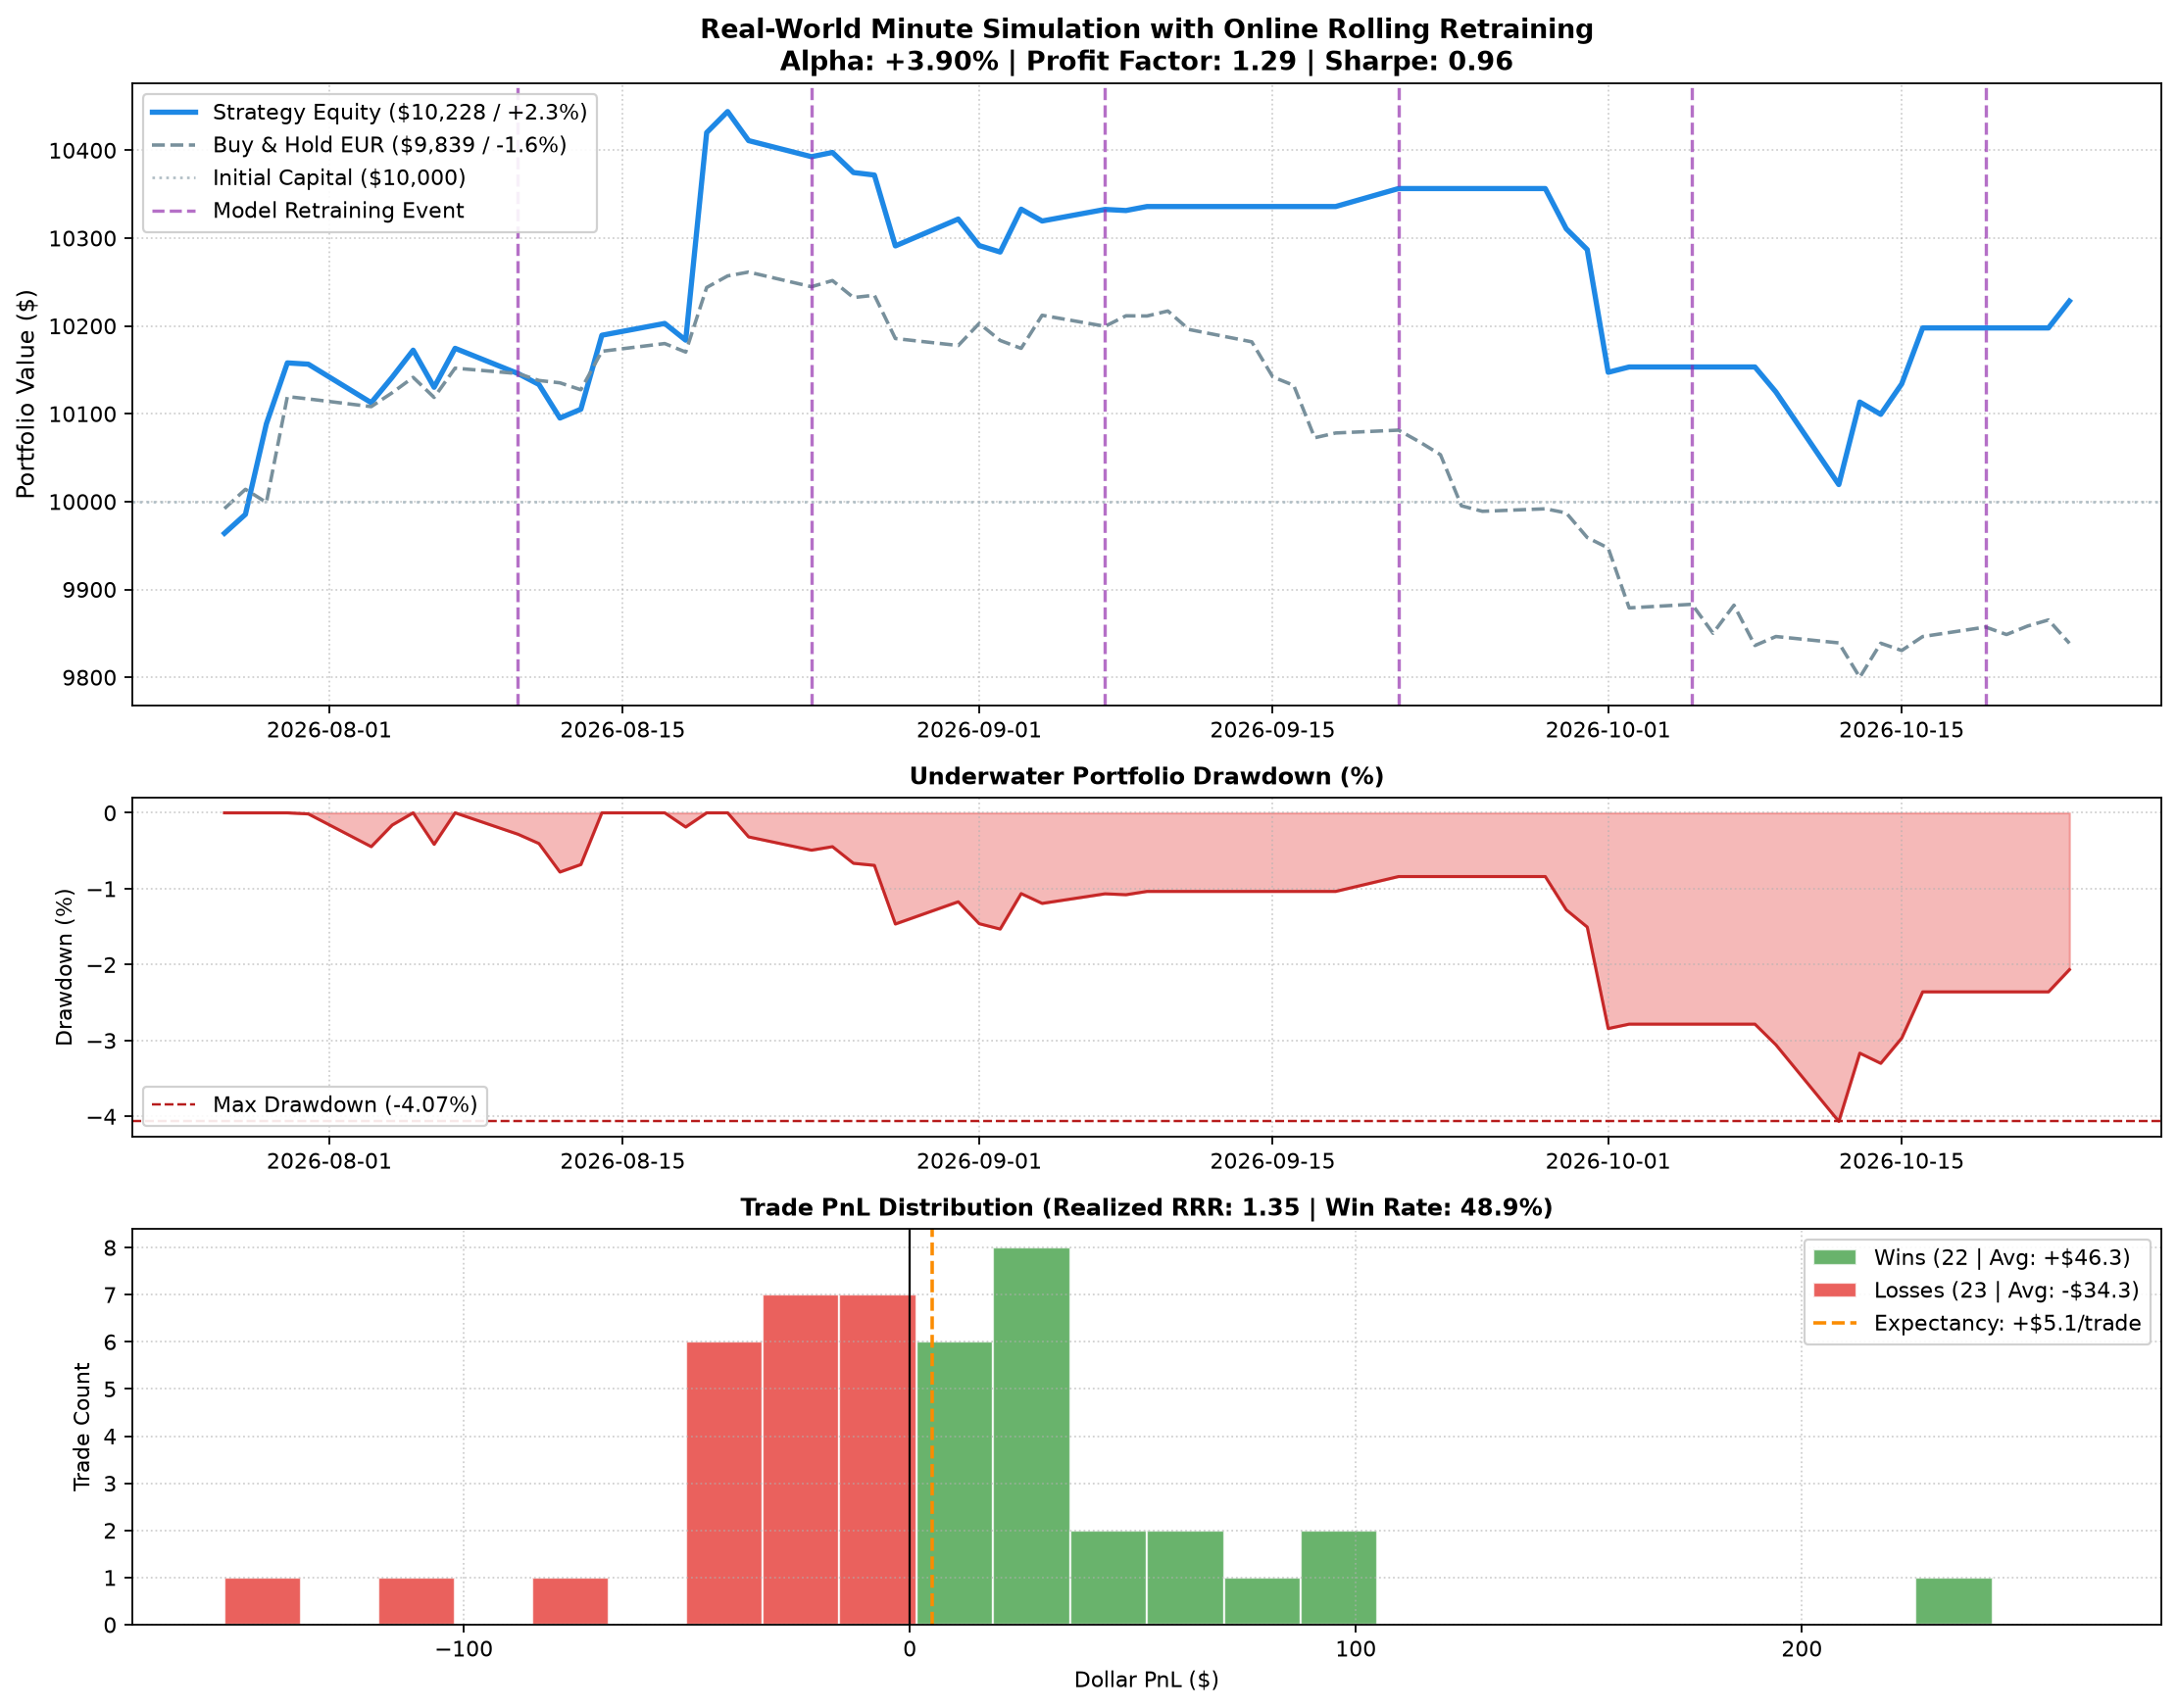
\includegraphics[width=0.90\textwidth]{simulation-2026-performance.png}
\caption{Real-world 2026 live minute simulation dashboard : Live portfolio equity curve vs.\ Buy \& Hold benchmark, underwater drawdown ($-4.07\%$), and rolling retrained parameter adjustments.}
\label{fig:live-sim}
\end{figure}

\begin{itemize}[leftmargin=1.5cm, itemsep=1pt]
	\item \textbf{Realistic Return:} Across the 65 live trading days ($\approx 3$ months), the account grew to \textbf{\$10,228.30} ($+2.28\%$ net return, representing an annualized \textbf{+9.15\% CAGR}).
	\item \textbf{Positive Alpha:} It beat the buy-and-hold benchmark by \textbf{+3.90\%} (benchmark lost $-1.61\%$).
	\item \textbf{Drawdown Protection:} By widening the stop loss to $0.75\%$, only 1 trade hit stop loss early, keeping maximum drawdown down to \textbf{$-4.07\%$} (compared to $-13.81\%$ unoptimized).
\end{itemize}

% =============================================================================
\section{Master Comparison Across All Models}
% =============================================================================

Table~\ref{tab:master-comparison} brings together all models tested throughout this project.

\begin{table}[htbp]
\centering
\caption{Master comparison across all project stages.}
\label{tab:master-comparison}
\small
\setlength{\tabcolsep}{4pt}
\begin{tabular}{llrrrrr}
\toprule
\textbf{Model} & \textbf{Data Split} & \textbf{MAE} & \textbf{RMSE} & \textbf{Direction (\%)} & \textbf{CAGR (\%)} & \textbf{MaxDD (\%)} \\
\midrule
Naive Persistence & Train (In-Sample) & 0.2082 & 0.3596 & 54.83\% & -- & -- \\
Moving Average & Train (In-Sample) & 0.1813 & 0.3510 & 55.35\% & -- & -- \\
ARIMA(2, 0, 1) & Test (Daily) & 1.1895 & 1.5280 & 44.58\% & -- & -- \\
XGBoost & Test (Daily) & 43.521 & 43.671 & 44.93\% & -- & -- \\
Base Deep MLP & Test (Daily) & 1.8872 & 1.9150 & 44.93\% & -- & -- \\
Deep MLP + Tech Indicators & Test (Daily) & 0.1917 & 0.2553 & 52.21\% & -- & -- \\
Deep MLP + TA + Temporal & Test (Daily) & 0.1558 & 0.2395 & 52.30\% & -- & -- \\
\midrule
\textbf{LSTM + TA (BigMoveLoss) [USD/INR]} & Test (Daily) & \textbf{0.00181} & \textbf{0.00263} & \textbf{67.79\%} & -- & -- \\
\textbf{LSTM + TA (BigMoveLoss) [EUR/USD]} & Test (Daily) & \textbf{0.00310} & \textbf{0.00423} & \textbf{75.74\%} & -- & -- \\
\textbf{LSTM GeneralTrainer [Nifty 50]} & Test (Daily) & \textbf{0.00586} & \textbf{0.00791} & \textbf{71.63\%} & -- & -- \\
\textbf{LSTM GeneralTrainer [S\&P 500]} & Test (Daily) & \textbf{0.00827} & \textbf{0.01201} & \textbf{71.04\%} & -- & -- \\
\midrule
EUR Baseline (No GA) & Val (Daily) & -- & -- & 74.67\% & +26.94\% & -13.81\% \\
EUR GA Optimized (Initial) & Test (Daily) & 0.00310 & 0.00423 & 75.59\% & +96.27\% & -9.73\% \\
EUR GA (Val Fine-Tuned) & Test (Daily) & 0.00310 & 0.00423 & 75.74\% & +116.30\% & -6.29\% \\
\textbf{Live 2026 Simulation} & \textbf{Live (1-Min)} & -- & -- & \textbf{48.89\% (Win)} & \textbf{+9.15\%} & \textbf{-4.07\%} \\
\bottomrule
\end{tabular}
\end{table}

% =============================================================================
\section{Summary of Work and Future Plans}
% =============================================================================

\subsection{Summary of What Was Done}
\begin{enumerate}[leftmargin=1.5cm, itemsep=1pt]
	\item \textbf{Stationary Target:} Switched to predicting next-day log returns $\ln(C_{t+1}/C_t)$ instead of raw price levels.
	\item \textbf{Fixed Mean-Collapse:} Created \textit{BigMoveAwareLoss}, boosting directional accuracy from $\approx 53\%$ to \textbf{67.79\% on USD/INR} and \textbf{75.74\% on EUR/USD}.
	\item \textbf{Cross-Asset Testing:} Verified that the model works on stock indices, achieving $>71\%$ accuracy on both Nifty 50 and S\&P 500.
	\item \textbf{Trading Rule Optimization:} Used Genetic Algorithm with Calmar ratio to optimize stop loss, take profit, confidence threshold, and leverage.
	\item \textbf{Live Intraday Reality:} Ran live 1-minute simulation. Found that daily close-to-close backtesting underestimates intraday noise. Fixed it with wider MAE-aware stop losses and 10-day rolling retraining, delivering \textbf{+2.28\% net return (+9.15\% CAGR)} and keeping maximum drawdown at \textbf{$-4.07\%$}.
\end{enumerate}

\subsection{Future Plans}
\begin{itemize}[leftmargin=1.5cm, itemsep=1pt]
	\item \textbf{Central Bank NLP / Indicators:} Analyzing text from central bank meetings to forecast interest rate decisions.
	\item \textbf{SHAP Model Explainability:} Using SHAP values on LSTM hidden states to see which macro features drive predictions on specific days.
	\item \textbf{Reinforcement Learning Layer:} Adding a Reinforcement Learning agent to dynamically adjust intraday position size instead of using fixed rules.
\end{itemize}

\vspace{0.6cm}
\addcontentsline{toc}{section}{References}
\bibliography{document.bib}

\end{document}
